%
% teil1.tex -- Beispiel-File für das Paper
%
% (c) 2020 Prof Dr Andreas Müller, Hochschule Rapperswil
%
% !TEX root = ../../buch.tex
% !TEX encoding = UTF-8
%
\section{Approximative geradlinige Bewegung
\label{geradlinig:section:approximative_geradlinig}}
\kopfrechts{Approximative geradlinige Bewegung}
Der erste approximative geradlinige Mechanismus war derjenige von James Watt, 
den er im Jahr 1784 patentieren liess.
In Abbildung~\ref{fig:watts_link} ist der Mechanismus vereinfacht 
dargestellt.
\begin{figure}[htbp]
    \centering
    \begin{minipage}{0.32\textwidth}
        \centering
        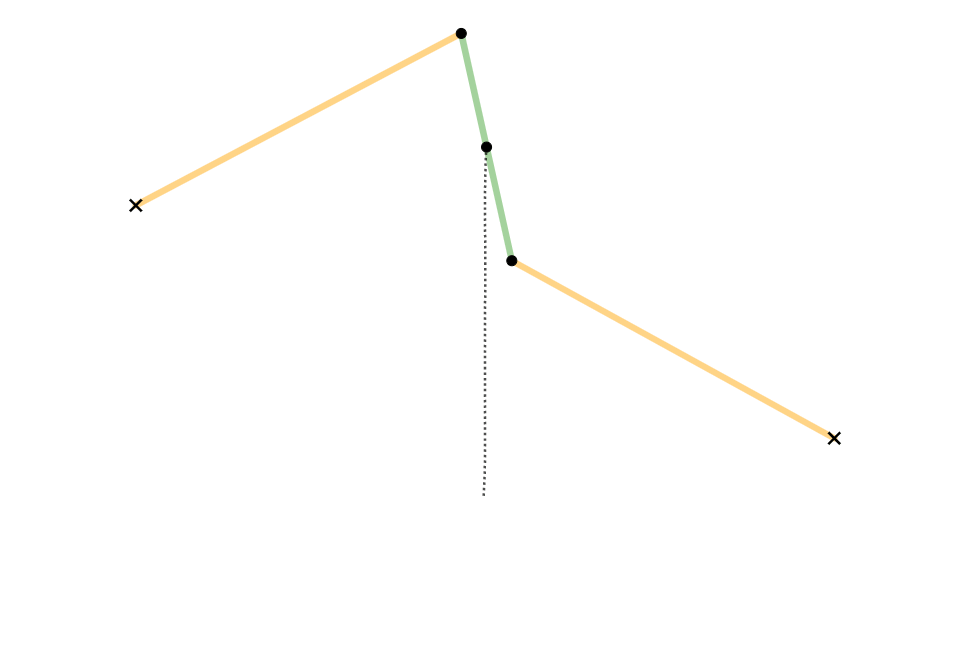
\includegraphics[width=\textwidth]{papers/geradlinig/figures/watts_linkage1.png}
    \end{minipage}
    \hfill
    \begin{minipage}{0.32\textwidth}
        \centering
        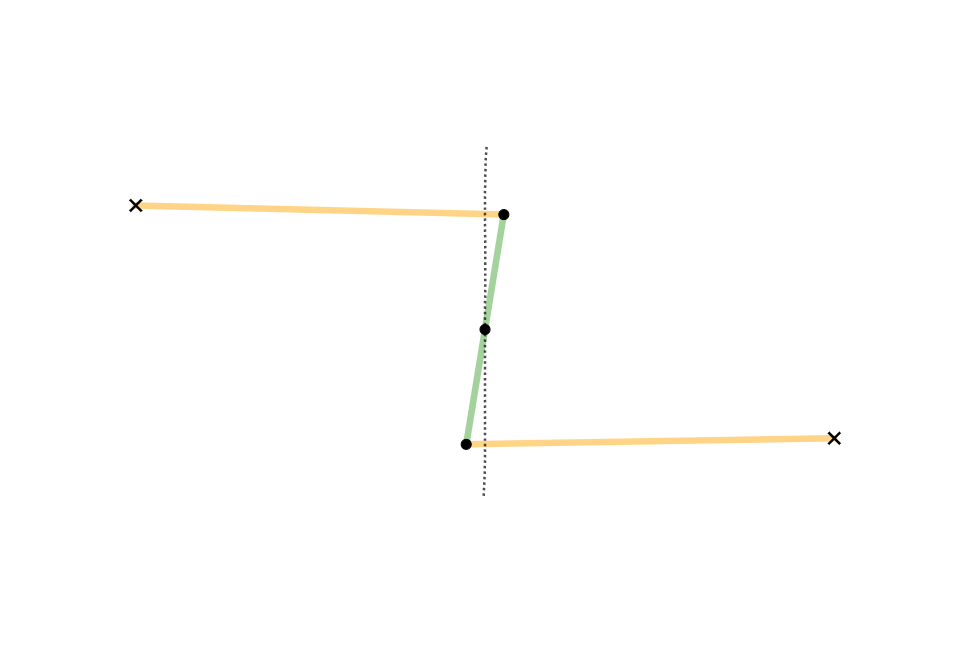
\includegraphics[width=\textwidth]{papers/geradlinig/figures/watts_linkage2.png}
    \end{minipage}
    \hfill
    \begin{minipage}{0.32\textwidth}
        \centering
        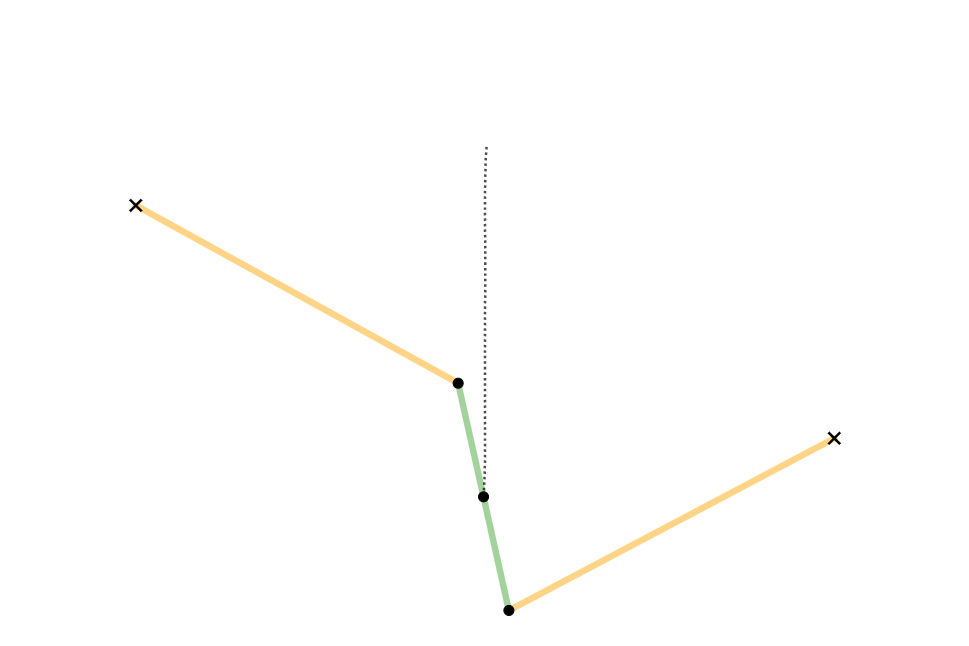
\includegraphics[width=\textwidth]{papers/geradlinig/figures/watts_linkage3.png}
    \end{minipage}
    \caption{Der Mechanismus von Watt~\cite{watt_linkage}.}
    \label{fig:watts_link}
\end{figure}

Die beiden gelben Gelenke müssen zwingend die gleiche Länge besitzen.
Das grüne Gelenk verbindet anschliessend die beiden Endpunkte 
der gelben Gelenke.
Dabei entsteht nur eine approximative Gerade, da der erzeugte Pfad 
nur in einem begrenzten Bereich nahezu geradlinig ist.
Der vollständige erzeugte Pfad entspricht einer Wattschen Kurve.
Ein Spezialfall der Wattschen Kurve ist in Abbildung~\ref{fig:lemniskate} 
dargestellt, bei welcher eine Lemniskate von Bernoulli entsteht.
In derselben Abbildung ist ersichtlich, 
dass der Pfad nur im Zentrum einer Geraden entspricht.
\begin{figure}[htbp]
    \centering
    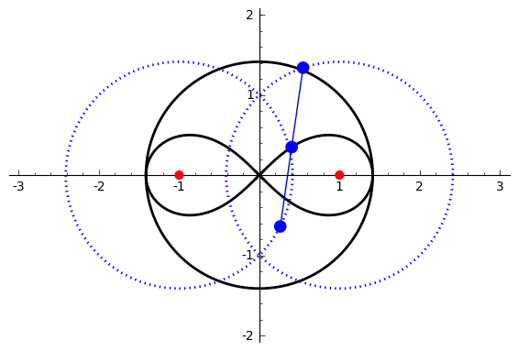
\includegraphics[width=0.5\textwidth]{papers/geradlinig/figures/lemniskate.png}
    \caption{Lemniskate von Bernoulli als Spezialfall der Wattschen Kurve~\cite{watt_curve}.}
    \label{fig:lemniskate}
\end{figure}

Ein weiteres Beispiel ist der Chebyshev-Mechanismus, 
welcher in Abbildung~\ref{fig:chebyshev_link} dargestellt ist.
Dieser besitzt die gleiche Anzahl an Gelenken wie der Watts-Mechanismus, 
verwendet jedoch eine andere Anordnung, 
um eine Rotationsbewegung in eine geradlinige Bewegung umzuwandeln.
Dabei gelten jedoch strengere Bedingungen für 
die Abmessungen der einzelnen Gelenke.
Das Verhältnis der gelben Gelenklänge zur blauen beträgt $2.5:1$.
Weitere Mechanismen, welche approximative geradlinige Bewegungen erzeugen, 
sind in~\cite{wiki_straight_line} aufgeführt.
\begin{figure}[htbp]
    \centering
    \begin{minipage}{0.32\textwidth}
        \centering
        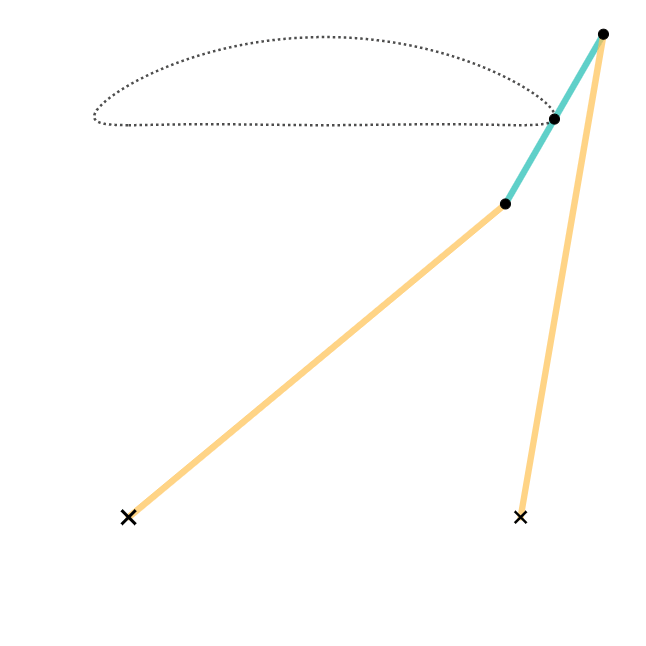
\includegraphics[width=\textwidth]{papers/geradlinig/figures/chebyshev_linkage1.png}
    \end{minipage}
    \hfill
    \begin{minipage}{0.32\textwidth}
        \centering
        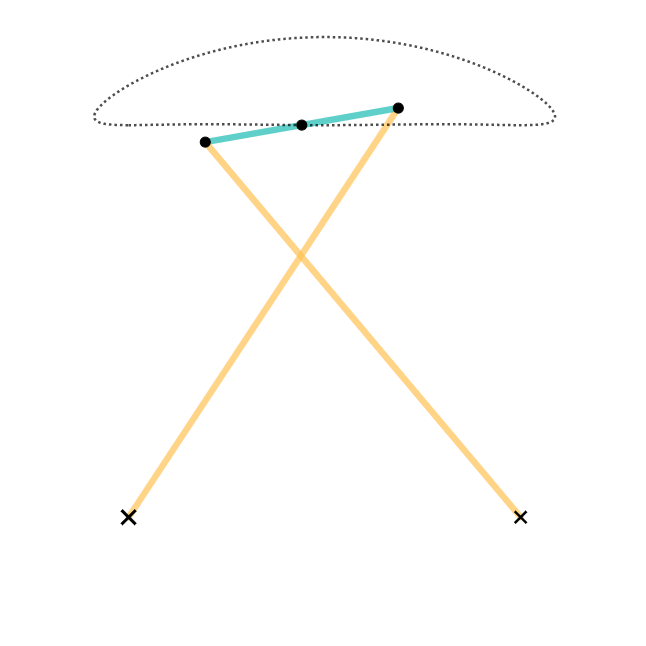
\includegraphics[width=\textwidth]{papers/geradlinig/figures/chebyshev_linkage2.png}
    \end{minipage}
    \hfill
    \begin{minipage}{0.32\textwidth}
        \centering
        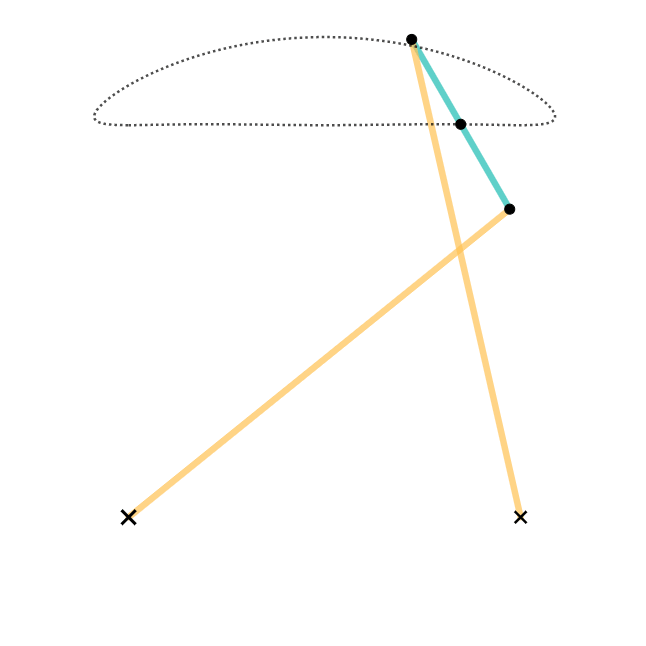
\includegraphics[width=\textwidth]{papers/geradlinig/figures/chebyshev_linkage3.png}
    \end{minipage}
    \caption{Der Mechanismus von Chebyshev~\cite{chebyshev_linkage}.}
    \label{fig:chebyshev_link}
\end{figure}

